% Packages & Document Configurations
\documentclass{IEEEtran}
\usepackage{graphicx}
\usepackage{float}
\usepackage{url}
\usepackage{amsmath}

\begin{document}

% Title
\title{Diet Type Prediction using Neural Networks}

\author{
    \IEEEauthorblockN{Awwab A. Samad}\\
    \IEEEauthorblockA{Department of Computer Engineering\\
    Information Technology University, Lahore, Pakistan\\
    Email: bsce21002@itu.edu.pk}
}

\date{\today}

\maketitle

% Abstract
\begin{abstract}
    In today's era of personalized medicine, the importance of tailored dietary recommendations for individuals with specific health conditions cannot be overstated. This project aims to utilize machine learning algorithms, particularly Neural Networks (MLP), to provide personalized dietary recommendations based on individuals' medical data. The proposed scheme involves training an MLP model on a dataset containing various medical parameters, such as BMI, blood glucose levels, and cholesterol levels, to predict a sequence of binary values representing dietary requirements. This document presents a detailed overview of the project, including the dataset, methodology, network architecture, implementation setup, and performance evaluation.
\end{abstract}

% Introduction
\section{Introduction}
With the increasing prevalence of chronic diseases such as diabetes, cardiovascular disorders, and obesity leading to substantial morbidity and mortality rates, there is a growing need for effective strategies to manage and prevent these conditions through lifestyle interventions, especially diet modification. However, devising personalized dietary plans that cater to individuals' unique medical profiles can be challenging, requiring a comprehensive understanding of their health status and nutritional requirements. Traditional approaches to dietary recommendation often rely on general guidelines and manual assessment by healthcare professionals, which may not fully account for individual variability and evolving health conditions often hindering effective disease prevention strategies.

In recent years, machine learning techniques have emerged as promising tools for personalized healthcare, offering the potential to analyze large volumes of medical data and extract meaningful insights to inform clinical decision-making. By leveraging algorithms such as neural networks, which are capable of learning complex, nonlinear patterns from data, it becomes possible to develop predictive models that can tailor dietary recommendations to each individuals' needs.

This project seeks to explore the feasibility of using Multi-Layer Perceptrons (MLP) to generate personalized dietary recommendations based on individuals' medical data. By training an MLP model on a diverse dataset comprising various medical parameters and corresponding dietary recommendations, we aim to analyze key risk factors and biomarkers associated with chronic diseases and develop a predictive system capable of providing optimal dietary choices for individuals that could ultimately encourage individuals to make healthier dietary choices and reduce their risk of chronic diseases.
% Proposed Scheme
\section{Proposed Scheme}
The proposed scheme of this project included 5 main phases for developing a diet recommendation system using machine learning. Here’s a brief explanation of the steps.

\begin{enumerate}
    \item \textbf{Data Collection}: This step involved collecting the data from online websites.
    \item \textbf{Data Preprocessing}: This step involved organizing the dataset, extracting the input features needed, and separating the data to be used in the training, validation, and testing phases.
    \item \textbf{Model Development}: This step involved selecting a machine learning technique, Multi-layer Perceptron and neural networks in our example, setting up the network architecture (input, hidden, and output neurons), and training the network to learn the relationship between inputs and outputs with the help of our training data.
    \item \textbf{Model Testing}: This step involved validating and testing our trained neural network with the help of our testing data.
    \item \textbf{Performance Evaluation}: This step involved analyzing the performance of the trained neural network through accuracy and loss graphs by comparing predicted vs actual outputs to evaluate how accurate our model is.
\end{enumerate}

\begin{figure}
    \centering
    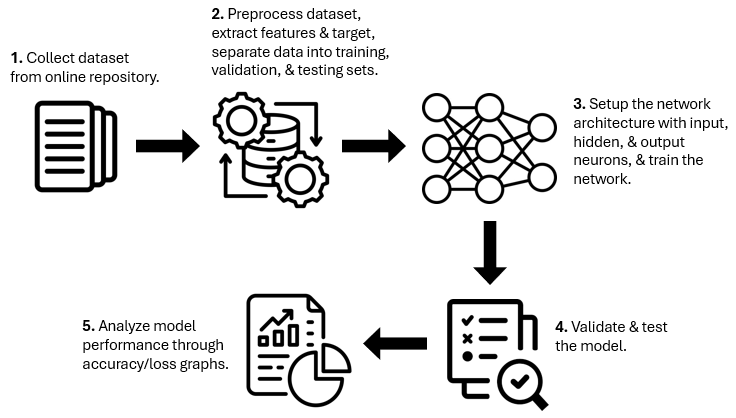
\includegraphics[width=\linewidth]{Figures/proposed scheme 2.png}
    \caption{Illustration of the proposed scheme}
\end{figure}
% Implementation
\section{Implementation}
The implementation process involved several key steps, including dataset acquisition, neural network model development, training and testing, and evaluation of results.

\subsection{Dataset Description}
The dataset utilized in this project was obtained from Kaggle \cite{metabolic_syndrome}. The dataset consists of a total of 2303 entries and contains medical information of various anonymous patients which are the input features that will be used to train our neural network.

Here is a brief description of the 9 input features used:

\begin{itemize}
    \item \textbf{Sex}: The gender of the individual (e.g., male or female).
    
    \item \textbf{WaistCirc}: The waist circumference of the individual, often used as a measure of abdominal obesity.
    
    \item \textbf{BMI}: Body Mass Index, calculated as the weight in kilograms divided by the square of the height in meters.
    
    \item \textbf{UrAlbCr}: Urinary Albumin-to-Creatinine Ratio ,a measure used to assess kidney function and detect signs of chronic kidney disease (CKD).
    
    \item \textbf{SerumUricAcid}: Serum Uric Acid level, a measure of uric acid concentration in the blood. Elevated levels will indicate conditions of gout and kidney disease in our project.
    
    \item \textbf{Fasting BGL}: Fasting Blood Glucose Level, the level of glucose in the blood after an overnight fast. It is will be used to diagnose diabetes and monitor blood sugar control in our project.
    
    \item \textbf{HDL}: High-Density Lipoprotein, cholesterol, often referred to as "good" cholesterol. Higher levels are associated with a reduced risk of heart disease.
    
    \item \textbf{Triglycerides}: Triglyceride levels in the blood, a type of fat found in the bloodstream. Elevated levels may increase the risk of hypertriglyceridemia which can lead to heart disease.
    
    \item \textbf{Bias}: We will additionally be adding a bias term or intercept in the neural network model to represent the constant term added to the weighted sum of input features.
\end{itemize}

Additionally, the dataset includes the target output, which is a sequence of 11 binary values representing dietary recommendations for the patient that a registered dietitian provided for us. The sequence order corresponds to the following diet types:
\begin{itemize}
    \item \textbf{LoSc}: Low simple carbohydrates
    \item \textbf{LoPrt}: Low protein
    \item \textbf{LoSF}: Low saturated fat
    \item \textbf{LoRM}: Low red meat
    \item \textbf{LoLgm}: Low legume
    \item \textbf{LoNa}: Low sodium
    \item \textbf{LoP}: Low phosphorus
    \item \textbf{HiUF}: High unsaturated fats
    \item \textbf{HiC}: High vitamin C
    \item \textbf{HiD}: High vitamin D
    \item \textbf{HiFib}: High fiber
\end{itemize}
For example, the sequence "1011101111" indicates that the patient should follow a diet that is low in simple carbohydrates, saturated fat, red meat, legume, sodium, phosphorus, and high in unsaturated fats, vitamin C, vitamin D, and fiber.

The diseases targeted for diet recommendation in this project include chronic kidney disease (CKD), diabetes, gout, hypertriglyceridemia (HTAG), and obesity. The severity of HTAG and obesity is indicated by levels 1 and 2, respectively. 

\subsection{Software and Hardware}
Here is an overview of the hardware and software tools required for the implementation of the project.
\newline\newline\textbf{Software:}
\begin{itemize}
    \item Programming Language: MATLAB R2020a
    \item Machine Learning Framework: Neural Network Toolbox
    \item Development Environment: MATLAB workspace
    \item Operating System: Windows 10
    \item Spreadsheet Software: Microsoft Excel (for dataset preprocessing and analysis)
\end{itemize}

\noindent\textbf{Hardware:}\newline
A computer with a decent processor and RAM to train the neural network.\\\\
\textbf{PC Specifications:}\\
\textbf{Processor:} i5-5200U CPU @2.20GHz\\
\textbf{RAM:} 16GB RAM DDR3\\
\textbf{Storage:} 1TB SSD Drive\\

\subsection{Neural Network Architecture}
The neural network architecture employed in this project is designed to process input features and generate corresponding output predictions. It comprises multiple layers of interconnected neurons, each serving a specific function in the learning process.

\begin{itemize}
\item \textbf{Input Neurons:} The neural network consists of 8 input neurons, representing the input features extracted from the dataset. Additionally, a bias neuron is included to account for any potential bias in the data which ensures that the network can adapt to variations in the input data. Hence, making a total of 9 input neurons.

\item \textbf{Output Neurons:} There are 11 output neurons in the network, corresponding to the target output of 11 binary values representing dietary recommendations. Each output neuron produces a binary output indicating the presence or absence of a specific dietary recommendation. For example, for the case of LoPrt, 1 indicates a recommended low protein diet and a 0 indicated not recommended.

\item \textbf{Hidden Neurons:} A hidden layer with 10 neurons is incorporated to facilitate the extraction of complex patterns and relationships within the input data. This number of hidden neurons was chosen to provide the network with sufficient capacity to learn dataset.

\item \textbf{Activation Function:} The sigmoidal activation function is used in the hidden layer which introduces non-linearity into the network's computations, enabling it to model complex relationships between input features and output predictions. It ensures that the output of each neuron is bounded between 0 and 1. The sigmoidal activation function is given by the formula:
\begin{equation}
    \sigma(x) = \frac{1}{1 + e^{-x}}
\end{equation}
\end{itemize}

\begin{figure}[!htpb]
    \centering
    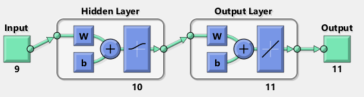
\includegraphics[width=\linewidth]{Figures/Neural Network.png}
    \caption{The implemented neural network model showing the number of input, hidden, and output neurons being utilized.}
\end{figure}

\subsection{Model Summary}
The Input layer has an output shape of (None, 9), representing a flexible batch size and 9 neurons. It doesn't contain any trainable parameters as it simply passes through the input data.

The neural network architecture includes two dense layers. The first dense layer has an output shape of (None, 10), indicating a flexible batch size and 10 neurons. It contains 90 parameters, calculated as $(\text{input\_dim} \times \text{units}) + \text{units} = (8 \times 10) + 10 = 90$, where the input dimension is 9 (8 input features plus 1 bias neuron).

The second dense layer has an output shape of (None, 11), representing 11 neurons in the output layer for the binary output values. It contains 121 parameters, calculated as $(\text{previous\_layer\_units} \times \text{units}) + \text{units} = (10 \times 11) + 11 = 121$, where the previous layer has 10 neurons.

Overall, the total number of parameters in the network is 211, all of which are trainable, with no non-trainable parameters.

\begin{table}[h]
\centering
\normalsize % Increase the font size of the table
\begin{tabular}{|l|l|l|}
\hline
\textbf{Layer (type)} & \textbf{Output Shape} & \textbf{Param \#} \\ \hline
Input & (None, 9) & 0 \\ \hline
Hidden (Dense) & (None, 10) & 90 \\ \hline
Output (Dense) & (None, 11) & 121 \\ \hline
\end{tabular}
\vspace{0.5cm}

\small{
\raggedright{
\hspace{0.8cm}\textbf{Total params:} 211 \\
\hspace{0.8cm}\textbf{Trainable params:} 211 \\
\hspace{-3.5cm}\textbf{Non-trainable params:} 0
}
}
\vspace{0.5cm}
\caption{Neural Network Architecture Summary}
\label{tab:neural_network_architecture}
\end{table}

\subsection{Model Training}
For model development, the dataset was divided into three subsets: 70\% for training (1612 entries), 15\% for validation (345 entries), and 15\% for testing (346 entries). This split ensures that the model is trained on a majority of the data while allowing for evaluation on unseen data to assess generalization performance.

During the training process, we utilized 1000 epochs with a learning rate (Mu) of 0.001. A higher number of epochs allows the model to undergo more iterations, thereby improving its ability to learn complex patterns from the data. Similarly, a lower learning rate helps prevent overshooting of the optimal solution and promotes stable convergence during training. Additionally, we incorporated 100 validation checks to prevent overfitting. This approach ensures that the model achieves optimal convergence and generalization.


\begin{figure}[!htpb]
    \centering
    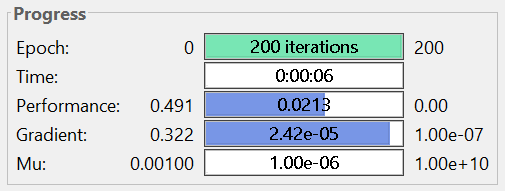
\includegraphics[width=\linewidth]{Figures/testing.png}
    \caption{Training the neural network with these parameters.}
    \label{fig:tcanther}
\end{figure}

During the training process, the neural network employs back propagation to update its weights iteratively. This process involves propagating error backwards through the network and calculating gradients of the loss function with respect to each weight. Specifically using gradient descent, weights are adjusted in small increments to minimize the error. This iterative adjustment continued across multiple epochs until the model converged, as evidenced by the gradient value decreasing to approximately $2.4189 \times 10^{-5}$ by the 200th epoch. At this point, with little to no change in gradients, the training process was stopped as the model had achieved satisfactory performance on the training data.

\begin{figure}[H]
    \centering
    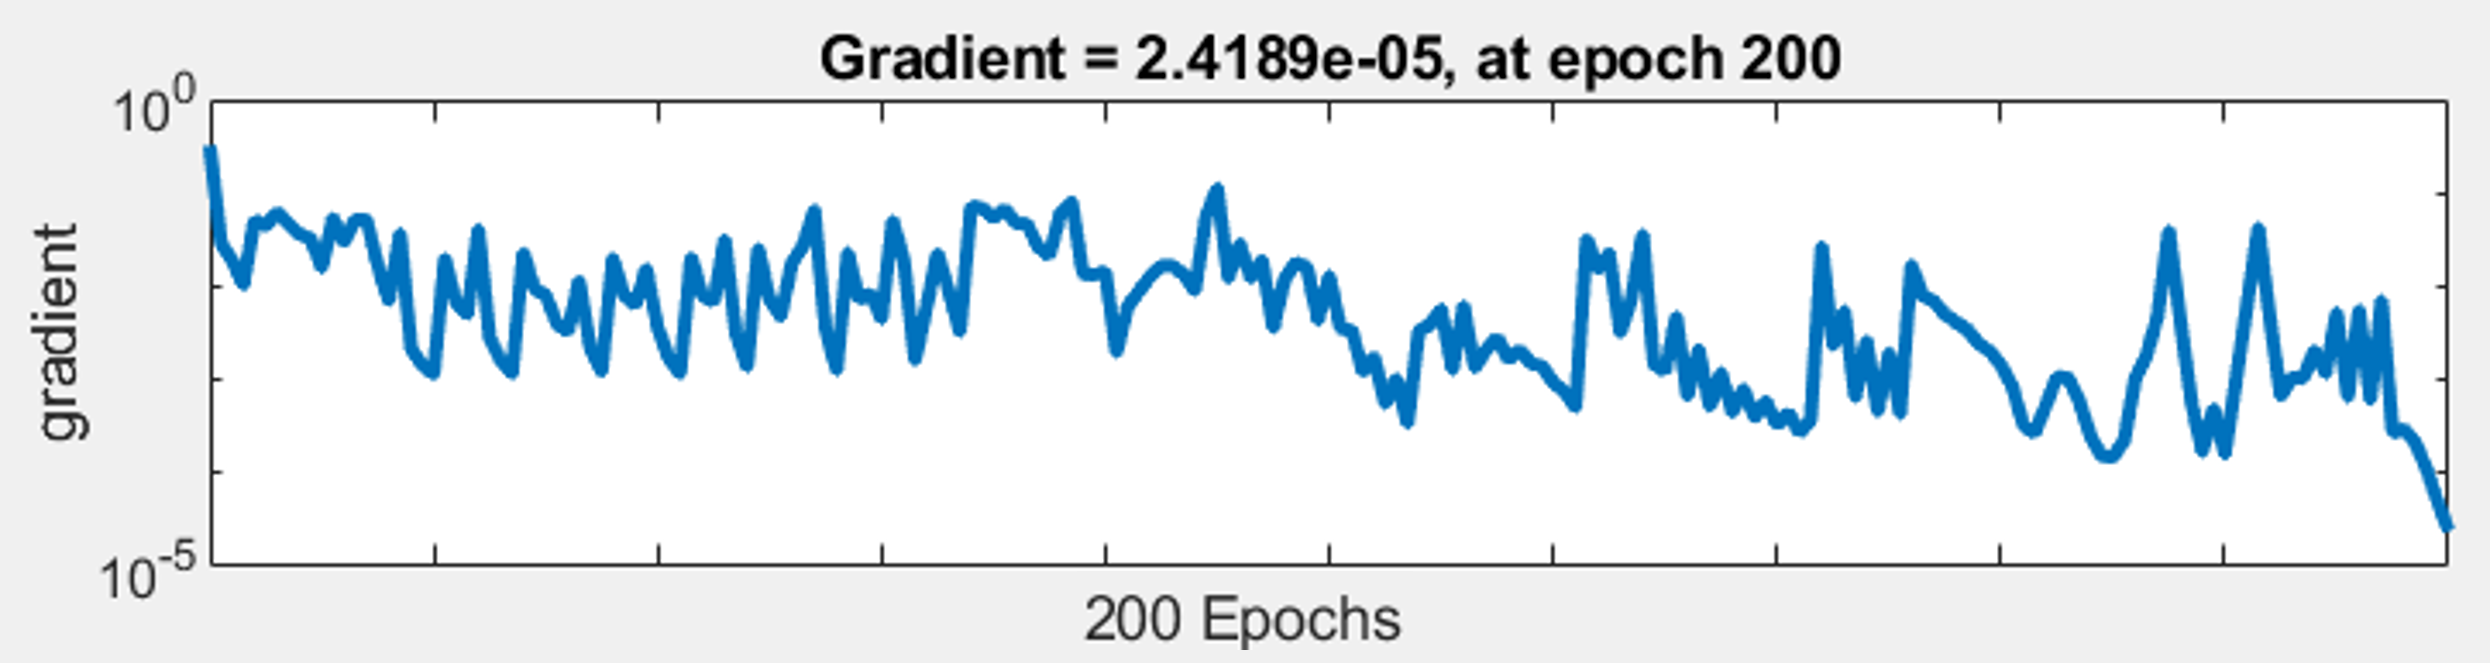
\includegraphics[width=\linewidth]{Figures/gradient2.png}
    \caption{Progression of gradient descent throughout the training iterations of the neural network.}
    \label{fig:tcanther}
\end{figure}

\subsection{Mean Squared Error}
A mean squared error graph was generated, which depicted a decreasing trend, indicating that the model's predictive accuracy improved steadily with each epoch until the curve started approaching towards a horizontal line. The lowest mean squared error achieved was 0.021327, suggesting that the model exhibited optimal performance in minimizing errors between predicted and actual outputs after 200 epochs.

\begin{figure}[!htpb]
    \centering
    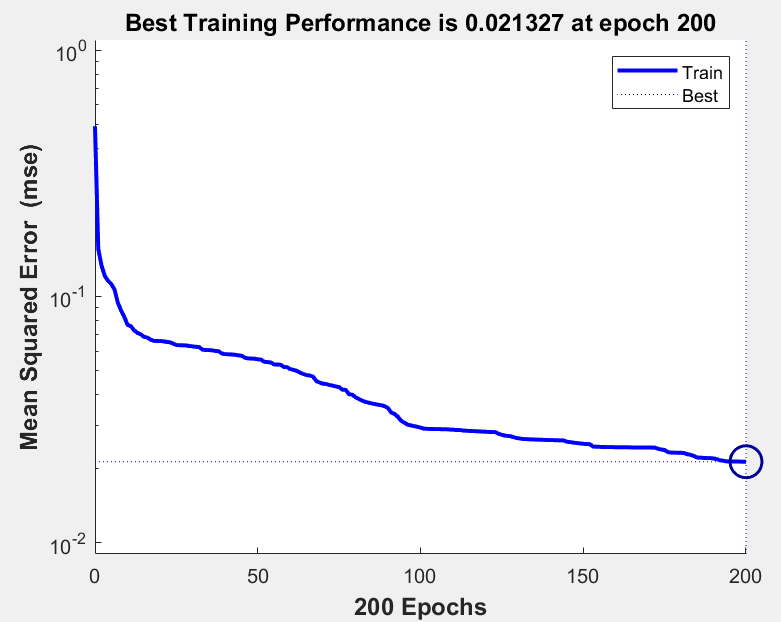
\includegraphics[width=\linewidth]{Figures/MSE2.png}
    \caption{Loss Graph: The decrease in MSE over epochs indicates that the model's predictions gradually converged towards the actual dietary recommendations as training progressed.}
\end{figure}

\subsection{Thresholds}
To ensure that the model's outputs are binary and align with the intended dietary recommendations, thresholds were incorporated into the output layer. These thresholds dictate the point at which the model classifies a recommendation as either present or absent based on the output neurons.
% Results
\section{Results and Evaluation}
Upon training the model using, we observed promising results in terms of accuracy. Tables and graphs were constructed of our validation and testing data with the help of MATLAB and Excel features to analyze the data and assess the accuracy of our trained model.

\subsection{Validation Results}
The success percentage of the diet recommendation system for the validation data was found to be very promising, yielding high rates of correct recommendations for each specific food/nutrient group. \textbf{Table II} summarizes the overall validation results, which presents the performance of dietary recommendations across different diet types (DT). Out of 345 total recommendations for each diet type, the model correctly predicted the majority, with a few incorrect predictions. The overall success rate, representing the accuracy of the recommendations, is remarkably high at 97.29\%.

\begin{table}[H]
    \centering
    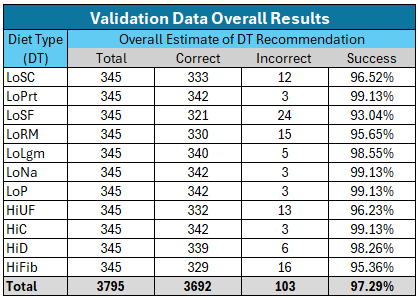
\includegraphics[width=\linewidth]{Figures/vdor.png}
    \caption{Results of the overall validation data.}
\end{table}

\textbf{Table III} shows the total number of instances where a diet type (DT) was recommended, along with the number of correct and incorrect predictions. Among the 1,674 recommendations, the model correctly identified 1,654 instances, achieving an overall accuracy of 98.81\%.
For instance, the diet type Low Simple Carbohydrates (LoSC) was recommended 278 times, with the model correctly predicting 277 of those recommendations, resulting in a success rate of 99.64\%. Similarly, the model achieved perfect accuracy of nearly 100\% for diet types such as Low Protein (LoPrt), Low Red Meat (LoRM), Low Sodium (LoNa), and Low Phosphorus (LoP). This high level of accuracy across various diet types demonstrates the model's effectiveness in making precise dietary recommendations when specific diet types are required.

\begin{table}[H]
    \centering
    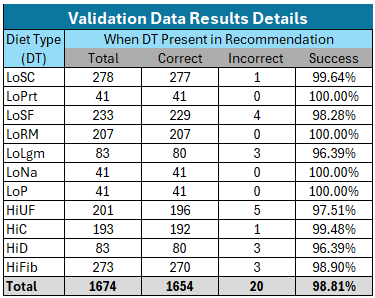
\includegraphics[width=\linewidth]{Figures/vdrdp.png}
    \caption{Results of the validation data when diet type was present in recommendation.}
\end{table}

\textbf{Table IV} shows the total number of instances where a diet type (DT) was not recommended. Among the 2121 recommendations, the model correctly identified 2038 instances, achieving an overall accuracy of 96.09\%.The incorrect predictions happen mostly when a diet type is not recommended to the patient (False Positive). LoSC, LoSF, LoRM and HiFib diet types have contributed to most of these false positives.


\begin{table}[H]
    \centering
    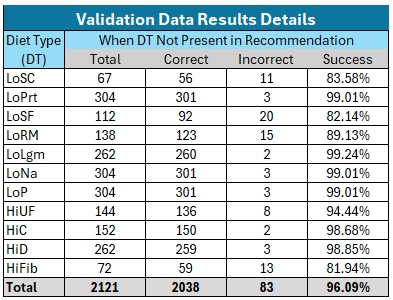
\includegraphics[width=\linewidth]{Figures/vdrdn.png}
    \caption{Results of the validation data when diet type was not present in recommendation.}
\end{table}

These values for accuracy also showed that the model tends to predict better when the diet type is recommended as opposed to when it isn't. A possible reason for this could be that fewer than needed training data was available for better prediction results.

\begin{table}[H]
    \centering
    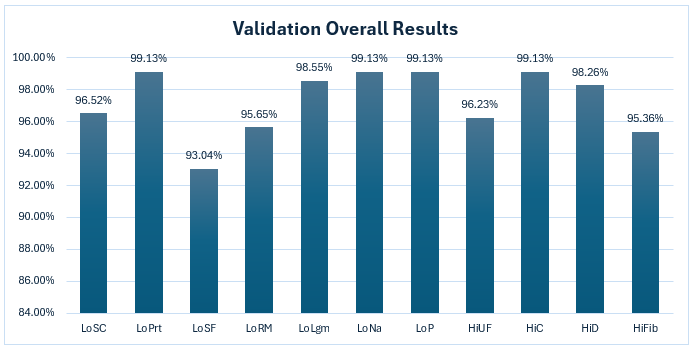
\includegraphics[width=\linewidth]{Figures/barv.png}
    \caption{Results of the overall validation data showing percentage accuracies for each diet type.}
\end{table}

\subsection{Testing Results}
Similarly, for the case of testing data, the overall accuracy of the results among a total of 3806 instances of the food groups combined with the testing data was 96.58\% as shown in \textbf{Table VI}. Success rate shows to vary from 91.04\% to 99.71\% within various diet type recommendations.


\begin{table}[H]
    \centering
    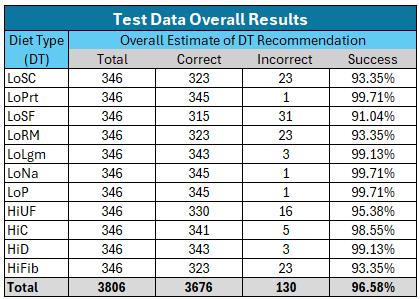
\includegraphics[width=\linewidth]{Figures/tdor.png}
    \caption{Results of the overall testing data.}
\end{table}

\textbf{Table VII} shows the total number of instances where a diet type (DT) was recommended, along with the number of correct and incorrect predictions. Among the 1,719 recommendations, the model correctly identified 1,687 instances, achieving an overall promising accuracy of 98.14\%.

\begin{table}[H]
    \centering
    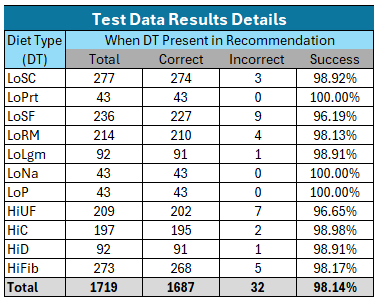
\includegraphics[width=\linewidth]{Figures/tdrdp.png}
    \caption{Results of the testing data when diet type was present in recommendation.}
\end{table}

Finally, \textbf{Table VIII} shows the total number of instances where a diet type (DT) was not recommended and among the 2087 recommendations, the model correctly identified 2038 instances, achieving an overall accuracy of 95.30\%, again reflecting the model's more accuracy in prediction when diet type is recommended as opposed to when it's not. Similar to the validation data, LoSC, LoSF, LoRM and HiFib have contributed to most of these false positives, meaning that these diet types got recommended to some patients by our neural network when they were actually not.


\begin{table}[H]
    \centering
    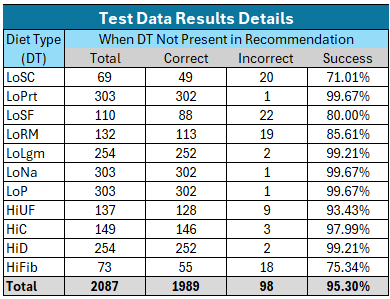
\includegraphics[width=\linewidth]{Figures/tdrdn.png}
    \caption{Results of the testing data when diet type was not present in recommendation.}
\end{table}

\subsection{Confusion Matrices}
A confusion matrix for the validation results show in \textbf{Fig. 6} was also made indicating that the model has a high accuracy of 97.2\%, correctly predicting 1,654 instances where a diet type was recommended (true positives) and 2,038 instances where a diet type was not recommended (true negatives). There were 83 false positives and 20 false negatives, resulting in a precision of 95.2\% and a recall of 98.8\%.

\begin{figure}[H]
    \centering
    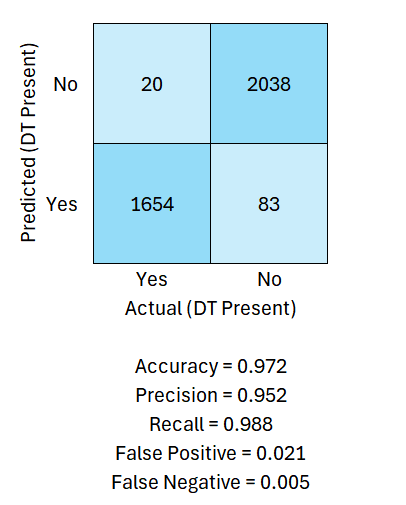
\includegraphics[width=\linewidth]{Figures/confusion_v.png}
    \caption{Confusion matrix compiling the overall validation results.}
\end{figure}

For the testing results, the confusion matrix show in \textbf{Fig. 7} shows an accuracy of 96.5\%, with 1,687 true positives and 1,989 true negatives. There were 98 false positives and 32 false negatives, resulting in a precision of 94.5\% and a recall of 98.1\%. The false positive rate was 2.5\%, and the false negative rate was 0.8\%.

These metrics indicate that the model performs consistently well on both validation and testing datasets, demonstrating high accuracy, precision, and recall in making dietary recommendations.


\begin{figure}[H]
    \centering
    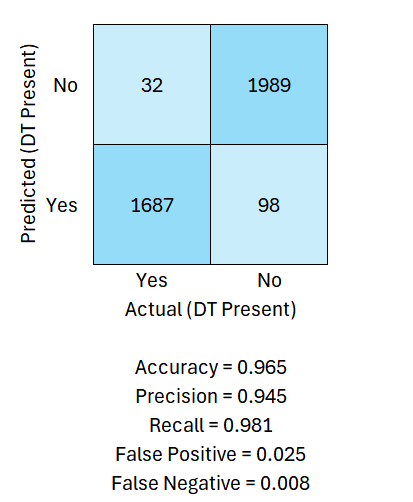
\includegraphics[width=\linewidth]{Figures/confusion_t.png}
    \caption{Confusion matrix compiling the overall testing results.}
\end{figure} 

\subsection{Neural Network Performance}
In conclusion, our neural network model performance was a success exhibiting well over 90\% accuracy. The network has behaved consistently when comparing the result of the testing and validating data as compared by \textbf{Table V} and \textbf{Table IX} and the confusion matrices.

\begin{table}[H]
    \centering
    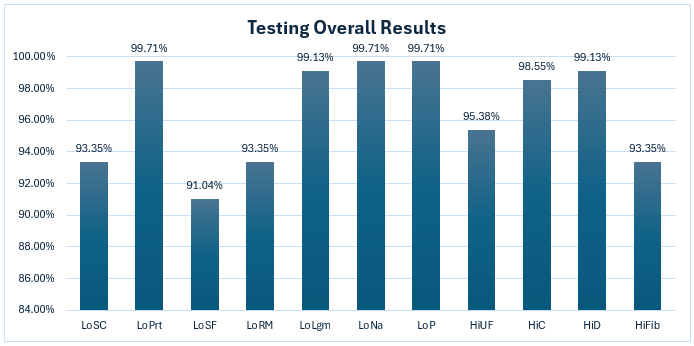
\includegraphics[width=\linewidth]{Figures/bart.png}
    \caption{Results of the overall testing data showing percentage accuracies for each diet type.}
\end{table} 




% Conclusion
\section{Conclusion}
This project presents a focused approach to dietary recommendation for individuals at risk of chronic diseases using a dataset of various medical data. By leveraging the neural network machine learning technique tailored to the available data, our solution aims to provide personalized food choices based on individual health profiles and encourage individuals to make better dietary choices, ultimately contributing to improved long term health and quality of life.

Future research work can proceed in the direction of better optimizing this neural network by adding an additional hidden layer and/or using different number of neurons in each hidden layer. Furthermore, more training data can be used to better train the network and achieve a better accuracy.

% References

\begin{thebibliography}{1}

\bibitem{metabolic_syndrome}
Albert Antony, "Metabolic Syndrome, A Comprehensive Dataset on Risk Factors and Health Indicators," [Online]. Available: \url{https://www.kaggle.com/datasets/antimoni/metabolic-syndrome}, Dec. 2023.

\bibitem{neural_network_matlab}
Technogineer, "How to use Neural network (NN) toolbox in MATLAB?," [Online Video]. Available: \url{https://www.youtube.com/watch?v=-R942VE-Jxk}, Apr. 26, 2020.

\bibitem{diabetes_prediction_dl}
Nuruzzuman Faruqui, "Diabetes Prediction using Deep Learning," [Online Video]. Available: \url{https://www.youtube.com/watch?v=8JDKL5RgPnY&list=PL9be9JpeQ7IP6jd0etq7quuUBYQYNXb50&index=12}, Sep. 23, 2021.

\bibitem{mlp_matlab}
Salman Mohagheghi, "Designing Multilayer Perceptron (MLP) Artificial Neural Networks in Matlab," [Online Video]. Available: \url{https://www.youtube.com/watch?v=RYL6_vDVWZs&t=377s}, Apr. 15, 2020.

\end{thebibliography}

\section*{Acknowledgements}
This project received support by the instructor of the Machine Learning course, Professor Dr. Tahira Mahboob, PhD and her Teaching Assistant, Ma'am Malaika Waheed at Information Technology University, Lahore, Pakistan.
It also received additional support from a registered dietition, Hodaa Samad.

\end{document}
